\documentclass[UTF8,aspectratio=169,11pt]{ctexbeamer}

\usetheme{Madrid}
\usecolortheme{default}
\usefonttheme{professionalfonts}

\usepackage{amsmath,amssymb}
\usepackage{booktabs,tabularx,array}
\usepackage{graphicx}
\usepackage{tikz}
\usetikzlibrary{arrows.meta,positioning,calc,fit}

\graphicspath{{figures/}}

\definecolor{nkuBlue}{RGB}{24,78,119}
\definecolor{nkuGreen}{RGB}{34,139,116}
\definecolor{nkuOrange}{RGB}{226,122,63}
\definecolor{nkuRed}{RGB}{190,69,61}
\definecolor{softGray}{RGB}{245,247,250}
\definecolor{textGray}{RGB}{55,65,81}

\setbeamercolor{structure}{fg=nkuBlue}
\setbeamercolor{frametitle}{fg=white,bg=nkuBlue}
\setbeamercolor{title}{fg=white,bg=nkuBlue}
\setbeamercolor{block title}{fg=white,bg=nkuBlue}
\setbeamercolor{block body}{bg=softGray,fg=textGray}
\setbeamercolor{alerted text}{fg=nkuRed}
\setbeamertemplate{navigation symbols}{}
\setbeamertemplate{footline}[frame number]
\setbeamertemplate{itemize item}{\color{nkuGreen}$\blacktriangleright$}
\setbeamertemplate{itemize subitem}{\color{nkuOrange}$\bullet$}

\newcommand{\key}[1]{\textcolor{nkuBlue}{\textbf{#1}}}
\newcommand{\warn}[1]{\textcolor{nkuRed}{\textbf{#1}}}

\title[协程技术调研]{协程技术调研：\\让等待不再占用线程}
\subtitle{从并发模型演进到底层实现与实验验证}
\author[匡航逸 / 2412235]{\texorpdfstring{匡航逸 \quad 2412235}{匡航逸 2412235}}
\institute{并行程序设计调研展示}
\date{\today}

\begin{document}

\begin{frame}
  \titlepage
\end{frame}

\begin{frame}{核心问题与展示主线}
  \begin{columns}[T,onlytextwidth]
    \begin{column}{0.48\textwidth}
      \begin{block}{核心判断}
        协程不是让计算变快，而是让 \key{等待变便宜}。
      \end{block}
      \vspace{0.6em}
      \begin{itemize}
        \item 大量请求处于 I/O 等待时，线程不应被长期占住。
        \item 协程把等待点变成可保存、可恢复的执行状态。
        \item 语言、运行时、操作系统必须共同配合。
      \end{itemize}
    \end{column}
    \begin{column}{0.48\textwidth}
      \begin{block}{内容主线}
        \begin{enumerate}
          \item 为什么从线程走到协程
          \item 协程底层如何暂停和恢复
          \item 常见应用范式如何落地
          \item 主流语言方案如何取舍
          \item 本机实验与工程边界
        \end{enumerate}
      \end{block}
    \end{column}
  \end{columns}
\end{frame}

\begin{frame}{问题背景：thread-per-request 的成本}
  \begin{columns}[T,onlytextwidth]
    \begin{column}{0.44\textwidth}
      \begin{itemize}
        \item 云服务中，单个请求常常大部分时间在等网络、磁盘、数据库。
        \item 若每个请求绑定一个 OS 线程，等待也会占用线程栈和调度实体。
        \item 线程池能限制线程数，但阻塞任务会把池子占满，导致排队。
      \end{itemize}
      \vspace{0.4em}
      \begin{block}{要解决的问题}
        不是“一个请求算得更快”，而是“十万请求同时等待时，系统还能撑住”。
      \end{block}
    \end{column}
    \begin{column}{0.54\textwidth}
      \centering
      \resizebox{\linewidth}{!}{%
      \begin{tikzpicture}[
        box/.style={draw,rounded corners=2pt,minimum height=0.72cm,align=center,font=\small},
        thread/.style={box,fill=nkuOrange!15,draw=nkuOrange!80!black},
        wait/.style={box,fill=nkuBlue!10,draw=nkuBlue!80!black},
        arrow/.style={-{Latex[length=2.2mm]},thick}
      ]
        \node[box,fill=softGray,minimum width=2.9cm] (req1) {请求 1};
        \node[box,fill=softGray,minimum width=2.9cm,below=0.32cm of req1] (req2) {请求 2};
        \node[box,fill=softGray,minimum width=2.9cm,below=0.32cm of req2] (req3) {请求 3};
        \node[font=\large,below=0.25cm of req3] (dots) {$\vdots$};
        \node[thread,right=1.35cm of req1,minimum width=2.8cm] (t1) {OS 线程};
        \node[thread,right=1.35cm of req2,minimum width=2.8cm] (t2) {OS 线程};
        \node[thread,right=1.35cm of req3,minimum width=2.8cm] (t3) {OS 线程};
        \node[wait,right=1.15cm of t2,minimum width=3.0cm,minimum height=2.8cm] (io) {等待 I/O\\线程仍被占用};
        \draw[arrow] (req1) -- (t1);
        \draw[arrow] (req2) -- (t2);
        \draw[arrow] (req3) -- (t3);
        \draw[arrow] (t1) -- (io.west |- t1);
        \draw[arrow] (t2) -- (io);
        \draw[arrow] (t3) -- (io.west |- t3);
        \node[below=0.5cm of io,align=center,font=\small,text=nkuRed] {高并发时：线程栈、切换、排队成本上升};
      \end{tikzpicture}
      }
    \end{column}
  \end{columns}
\end{frame}

\begin{frame}{并发模型的演进路线}
  \centering
  \resizebox{0.98\textwidth}{!}{%
  \begin{tikzpicture}[
    stage/.style={draw,rounded corners=3pt,minimum width=2.15cm,minimum height=1.0cm,align=center,font=\small,fill=softGray},
    arrow/.style={-{Latex[length=2mm]},thick,draw=textGray}
  ]
    \node[stage] (p) {多进程\\隔离强};
    \node[stage,right=0.38cm of p] (t) {多线程\\共享内存};
    \node[stage,right=0.38cm of t] (pool) {线程池\\控制数量};
    \node[stage,right=0.38cm of pool] (event) {事件驱动\\回调};
    \node[stage,right=0.38cm of event,fill=nkuGreen!13,draw=nkuGreen!80!black] (co) {协程\\async/await};
    \node[stage,right=0.38cm of co,fill=nkuOrange!13,draw=nkuOrange!85!black] (vt) {轻量线程\\Go / Java};

    \draw[arrow] (p) -- (t);
    \draw[arrow] (t) -- (pool);
    \draw[arrow] (pool) -- (event);
    \draw[arrow] (event) -- (co);
    \draw[arrow] (co) -- (vt);

    \node[below=1.1cm of t,align=center,font=\small,text=nkuRed] {问题：创建、栈空间、内核调度、阻塞排队};
    \node[below=1.1cm of co,align=center,font=\small,text=nkuGreen!55!black] {目标：保留顺序代码体验，同时具备异步 I/O 伸缩性};
  \end{tikzpicture}
  }

  \vspace{0.8em}
  \begin{block}{演进的本质}
    执行单元越来越轻，调度权越来越多地交给语言运行时；但真正的 I/O 事件仍由操作系统提供。
  \end{block}
\end{frame}

\begin{frame}{协程是什么：可暂停和恢复的函数}
  \begin{columns}[T,onlytextwidth]
    \begin{column}{0.46\textwidth}
      \begin{itemize}
        \item 普通函数：沿调用栈执行到返回。
        \item 协程：在 \texttt{await} / \texttt{co\_await} / \texttt{yield} 处挂起。
        \item 挂起时保存执行位置、局部变量、返回值或异常状态。
        \item 恢复时从挂起点之后继续执行。
      \end{itemize}
      \vspace{0.5em}
      \begin{block}{关键区别}
        协程不是异步 I/O 本身，而是异步控制流的一种表达方式。
      \end{block}
    \end{column}
    \begin{column}{0.52\textwidth}
      \centering
      \begin{tikzpicture}[
        node distance=0.62cm,
        box/.style={draw,rounded corners=2pt,minimum width=4.5cm,minimum height=0.72cm,align=center,font=\small},
        arrow/.style={-{Latex[length=2mm]},thick}
      ]
        \node[box,fill=softGray] (s0) {状态 0：入口到第一个 await};
        \node[box,fill=nkuBlue!9,below=of s0] (await1) {挂起点：保存协程帧};
        \node[box,fill=softGray,below=of await1] (s1) {状态 1：I/O 完成后继续};
        \node[box,fill=nkuBlue!9,below=of s1] (await2) {挂起点：注册 continuation};
        \node[box,fill=softGray,below=of await2] (end) {结束：返回结果 / 抛出异常};
        \draw[arrow] (s0) -- (await1);
        \draw[arrow] (await1) -- (s1);
        \draw[arrow] (s1) -- (await2);
        \draw[arrow] (await2) -- (end);
        \node[right=0.35cm of await1,font=\footnotesize,text=nkuGreen,align=left] {线程去执行\\其他 ready task};
        \node[right=0.35cm of await2,font=\footnotesize,text=nkuGreen,align=left] {等待事件\\唤醒};
      \end{tikzpicture}
    \end{column}
  \end{columns}
\end{frame}

\begin{frame}{底层机制：编译器状态机 + 运行时调度}
  \begin{columns}[T,onlytextwidth]
    \begin{column}{0.46\textwidth}
      \begin{itemize}
        \item 编译器把异步函数拆成状态机。
        \item 跨越挂起点仍存活的数据进入协程帧。
        \item 运行时保存 continuation，并在条件满足后恢复。
        \item C++20 暴露 \texttt{promise}、\texttt{coroutine\_handle}、awaiter 等底层接口。
      \end{itemize}
    \end{column}
    \begin{column}{0.52\textwidth}
      \centering
      \resizebox{\linewidth}{!}{%
      \begin{tikzpicture}[
        box/.style={draw,rounded corners=3pt,align=center,font=\small,minimum height=0.82cm},
        arrow/.style={-{Latex[length=2mm]},thick}
      ]
        \node[box,fill=softGray,minimum width=3.1cm] (src) {\texttt{async f()}\\源代码};
        \node[box,fill=nkuBlue!10,minimum width=3.2cm,right=0.9cm of src] (compiler) {编译器\\拆状态机};
        \node[box,fill=nkuGreen!12,minimum width=3.2cm,right=0.9cm of compiler] (frame) {协程帧\\状态 + 局部变量};
        \node[box,fill=nkuOrange!13,minimum width=3.2cm,below=0.9cm of compiler] (rt) {运行时\\ready queue / timer / I/O};
        \node[box,fill=softGray,minimum width=3.2cm,below=0.9cm of frame] (os) {操作系统\\epoll / kqueue / IOCP};

        \draw[arrow] (src) -- (compiler);
        \draw[arrow] (compiler) -- (frame);
        \draw[arrow] (frame) -- (rt);
        \draw[arrow,bend left=20] (rt) to (os);
        \draw[arrow,bend left=20] (os) to (rt);
      \end{tikzpicture}
      }
    \end{column}
  \end{columns}

  \vspace{0.5em}
  \begin{block}{一句话}
    协程“暂停”的本质，是把执行现场从线程栈搬到可保存、可恢复的数据结构中。
  \end{block}
\end{frame}

\begin{frame}{事件循环：等待不占线程的关键}
  \begin{columns}[T,onlytextwidth]
    \begin{column}{0.48\textwidth}
      \begin{itemize}
        \item \key{ready queue}：已经可以运行的任务。
        \item \key{timer heap}：定时器到期后唤醒任务。
        \item \key{I/O poller}：等待 fd、socket 或系统完成事件。
      \end{itemize}
      \vspace{0.3em}
      \begin{block}{运行流程}
        当前协程遇到未就绪 I/O 时挂起，线程立刻切到其他 ready task；I/O 完成后再把它放回队列。
      \end{block}
    \end{column}
    \begin{column}{0.50\textwidth}
      \centering
      \resizebox{\linewidth}{!}{%
      \begin{tikzpicture}[
        box/.style={draw,rounded corners=3pt,align=center,font=\small,minimum width=3.0cm,minimum height=0.82cm},
        arrow/.style={-{Latex[length=2mm]},thick}
      ]
        \node[box,fill=nkuGreen!12] (ready) at (0,1.75) {ready queue};
        \node[box,fill=softGray] (task) at (4.25,1.75) {运行一个 Task};
        \node[box,fill=nkuOrange!12] (wait) at (4.25,0) {await I/O / timer};
        \node[box,fill=nkuBlue!10] (poller) at (0,0) {I/O poller\\timer heap};

        \draw[arrow] (ready) -- node[above,font=\scriptsize] {取出任务} (task);
        \draw[arrow] (task) -- node[right,font=\scriptsize] {未就绪} (wait);
        \draw[arrow] (wait) -- node[below,font=\scriptsize] {注册等待} (poller);
        \draw[arrow] (poller) -- node[left,font=\scriptsize] {完成事件} (ready);
      \end{tikzpicture}
      }

      \vspace{0.6em}
      \footnotesize
      Linux 常见为 \texttt{epoll}，macOS/BSD 为 \texttt{kqueue}，Windows 为 IOCP。
    \end{column}
  \end{columns}
\end{frame}

\begin{frame}{应用范式：把并发写成可控控制流}
  \small
  \begin{columns}[T,onlytextwidth]
    \begin{column}{0.50\textwidth}
      \begin{block}{常见模式}
        \begin{itemize}
          \item \textbf{请求级协程}：一个请求一条可挂起控制流。
          \item \textbf{fan-out / fan-in}：并发访问多个下游，再汇总结果。
          \item \textbf{生产者--消费者}：异步队列连接爬取、解析、写入等阶段。
          \item \textbf{受限并发}：信号量、连接池、bounded queue 控制容量。
        \end{itemize}
      \end{block}
      \vspace{0.15em}
      \begin{block}{关键边界}
        协程让等待不占线程，但不会扩大下游容量；必须配合超时、取消和限流。
      \end{block}
    \end{column}
    \begin{column}{0.48\textwidth}
      \centering
      \resizebox{0.94\linewidth}{!}{%
      \begin{tikzpicture}[
        box/.style={draw,rounded corners=3pt,align=center,font=\small,minimum width=2.15cm,minimum height=0.72cm},
        arrow/.style={-{Latex[length=2mm]},thick}
      ]
        \node[box,fill=softGray] (req) at (0,1.6) {上层请求};
        \node[box,fill=nkuGreen!12] (a) at (3.2,2.6) {协程 A\\查缓存};
        \node[box,fill=nkuGreen!12] (b) at (3.2,1.6) {协程 B\\查数据库};
        \node[box,fill=nkuGreen!12] (c) at (3.2,0.6) {协程 C\\调下游};
        \node[box,fill=nkuBlue!10] (limit) at (6.2,1.6) {限流 / 超时\\取消传播};
        \node[box,fill=nkuOrange!12] (join) at (8.9,1.6) {汇总结果};
        \draw[arrow] (req) -- (a);
        \draw[arrow] (req) -- (b);
        \draw[arrow] (req) -- (c);
        \draw[arrow] (a) -- (limit);
        \draw[arrow] (b) -- (limit);
        \draw[arrow] (c) -- (limit);
        \draw[arrow] (limit) -- (join);
      \end{tikzpicture}
      }

      \vspace{0.25em}
      \scriptsize
      这类结构的目标是降低总等待时间，同时把资源上限写进程序结构。
    \end{column}
  \end{columns}
\end{frame}

\begin{frame}{主流语言支持：同一问题的不同取舍}
  \scriptsize
  \begin{tabularx}{\textwidth}{p{1.35cm}p{2.45cm}p{3.0cm}X}
    \toprule
    语言 & 编程接口 & 调度模型 & 适合场景与注意点 \\
    \midrule
    C++20 & \texttt{co\_await}, \texttt{co\_yield} & 标准提供 stackless coroutine 机制；事件循环由库实现 & 控制力强、开销可控；工程中需要选定 runtime / executor \\
    Go & \texttt{go f()}, channel & Goroutine 由 G-M-P runtime 映射到 OS 线程 & 服务端体验好；阻塞、GC、共享内存竞争仍要管理 \\
    Python & \texttt{async def}, \texttt{await}, \texttt{asyncio} & 单事件循环协作式调度 Task & 网络 I/O 友好；阻塞函数和 CPU 长任务会卡住事件循环 \\
    C\# & \texttt{async}/\texttt{await}, \texttt{Task} & 编译器状态机 + TaskScheduler / 线程池 continuation & 生态完整；注意上下文捕获、\texttt{Result/Wait} 死锁风险 \\
    Java 21 & Virtual Threads & JVM 用户态线程挂载到 carrier platform thread & 保留 thread-per-request 写法；不是 CPU 加速工具，pinning 需关注 \\
    \bottomrule
  \end{tabularx}

  \vspace{0.8em}
  \begin{block}{观察}
    C++ / Python / C\# 更像显式 async 控制流；Go / Java 更像由运行时托管的轻量级线程。
  \end{block}
\end{frame}

\begin{frame}{Go 与 Java：轻量级线程路线}
  \begin{columns}[T,onlytextwidth]
    \begin{column}{0.49\textwidth}
      \begin{block}{Go Goroutine}
        \begin{itemize}
          \item G：goroutine，用户态任务。
          \item M：machine，OS thread。
          \item P：processor，执行 Go 代码需要的调度资源。
        \end{itemize}
      \end{block}
      \centering
      \begin{tikzpicture}[
        box/.style={draw,rounded corners=2pt,align=center,font=\scriptsize,minimum width=1.3cm,minimum height=0.5cm},
        arrow/.style={-{Latex[length=1.6mm]},thick}
      ]
        \node[box,fill=nkuGreen!12] (g1) {G};
        \node[box,fill=nkuGreen!12,below=0.18cm of g1] (g2) {G};
        \node[box,fill=nkuGreen!12,below=0.18cm of g2] (g3) {G};
        \node[box,fill=nkuBlue!10,right=0.8cm of g2] (p) {P};
        \node[box,fill=nkuOrange!12,right=0.8cm of p] (m) {M\\OS 线程};
        \draw[arrow] (g1.east) -- (p.west);
        \draw[arrow] (g2.east) -- (p.west);
        \draw[arrow] (g3.east) -- (p.west);
        \draw[arrow] (p) -- (m);
      \end{tikzpicture}
    \end{column}
    \begin{column}{0.49\textwidth}
      \begin{block}{Java Virtual Thread}
        \begin{itemize}
          \item 仍是 \texttt{java.lang.Thread} 实例。
          \item 可在阻塞 I/O 处 unmount，释放 carrier thread。
          \item 适合保留同步风格的高并发服务。
        \end{itemize}
      \end{block}
      \centering
      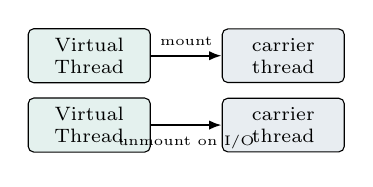
\begin{tikzpicture}[
        box/.style={draw,rounded corners=2pt,align=center,font=\scriptsize,minimum width=1.55cm,minimum height=0.5cm},
        arrow/.style={-{Latex[length=1.6mm]},thick}
      ]
        \node[box,fill=nkuGreen!12] (v1) {Virtual\\Thread};
        \node[box,fill=nkuGreen!12,below=0.18cm of v1] (v2) {Virtual\\Thread};
        \node[box,fill=nkuBlue!10,right=0.9cm of v1] (c1) {carrier\\thread};
        \node[box,fill=nkuBlue!10,right=0.9cm of v2] (c2) {carrier\\thread};
        \draw[arrow] (v1) -- node[above,font=\tiny] {mount} (c1);
        \draw[arrow] (v2) -- node[below,font=\tiny] {unmount on I/O} (c2);
      \end{tikzpicture}
    \end{column}
  \end{columns}

  \vspace{0.5em}
  \begin{block}{共同点}
    让程序员保留接近线程式的写法，由运行时把大量轻量任务复用到较少 OS 线程上。
  \end{block}
\end{frame}

\begin{frame}{实验设计：用 Python 验证协程边界}
  \begin{columns}[T,onlytextwidth]
    \begin{column}{0.48\textwidth}
      \begin{block}{等待型负载}
        2000 个任务，每个任务等待 5 ms，验证“等待是否占用线程”。
      \end{block}
      \begin{itemize}
        \item \textbf{asyncio}：\texttt{asyncio.sleep}，Task 挂起后回到事件循环。
        \item \textbf{ThreadPool}：\texttt{time.sleep}，等待时占用 worker。
        \item \textbf{Serial}：串行等待，作为基线。
      \end{itemize}
    \end{column}
    \begin{column}{0.48\textwidth}
      \begin{block}{CPU 密集负载}
        80 个纯 Python 循环任务，每个任务 120000 次整数更新。
      \end{block}
      \begin{itemize}
        \item 对比串行、\texttt{asyncio.gather} 和 8 worker 线程池。
        \item 用来约束结论：协程不是 CPU 加速工具。
      \end{itemize}
      \vspace{0.3em}
      \begin{block}{运行环境}
        \begin{itemize}
          \item Python 3.12.7
          \item Windows 本机环境
          \item 每组重复 5 次，图中展示均值与标准差
        \end{itemize}
      \end{block}
    \end{column}
  \end{columns}
\end{frame}

\begin{frame}{实验结果：等待变便宜，计算不变快}
  \begin{columns}[T,onlytextwidth]
    \begin{column}{0.64\textwidth}
      \centering
      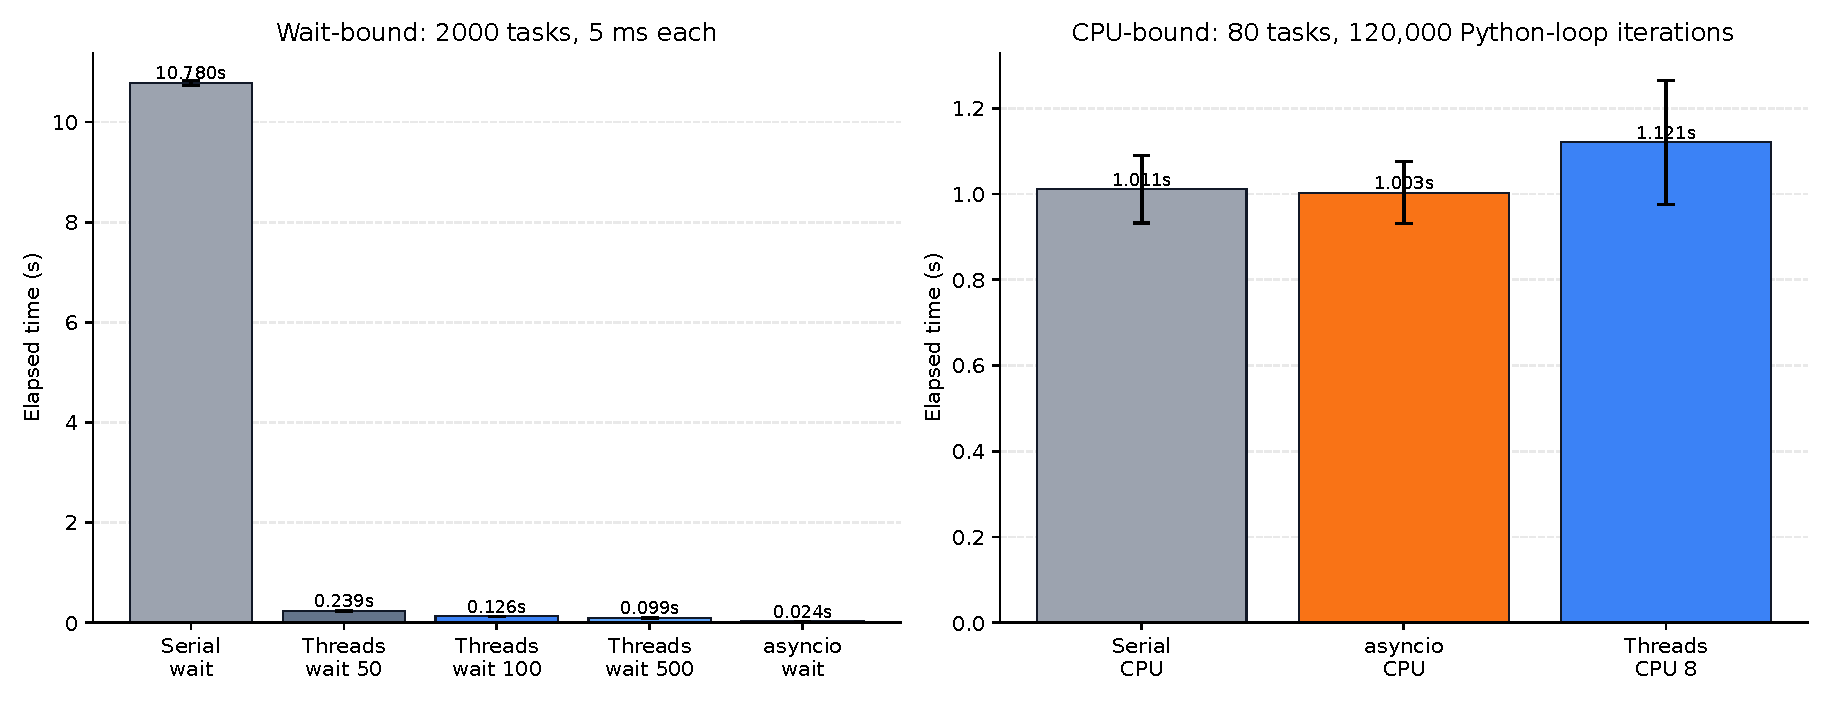
\includegraphics[width=\textwidth]{experiment_benchmarks.pdf}
    \end{column}
    \begin{column}{0.34\textwidth}
      \scriptsize
      \begin{tabular}{lr}
        \toprule
        等待型方案 & 平均耗时 \\
        \midrule
        Serial & 10.780 s \\
        Threads 50 & 0.239 s \\
        Threads 100 & 0.126 s \\
        Threads 500 & 0.099 s \\
        asyncio & 0.024 s \\
        \bottomrule
      \end{tabular}

      \vspace{0.7em}
      \begin{tabular}{lr}
        \toprule
        CPU 型方案 & 平均耗时 \\
        \midrule
        Serial & 1.011 s \\
        asyncio & 1.003 s \\
        Threads 8 & 1.121 s \\
        \bottomrule
      \end{tabular}
    \end{column}
  \end{columns}

  \vspace{0.3em}
  \begin{block}{解释边界}
    等待型任务中，协程挂起后不占 OS 线程；CPU 任务中，\texttt{asyncio} 与串行同量级，不能替代真正的并行计算。
  \end{block}
\end{frame}

\begin{frame}{工程边界：什么时候该用，什么时候不该用}
  \begin{columns}[T,onlytextwidth]
    \begin{column}{0.49\textwidth}
      \begin{block}{适合协程}
        \begin{itemize}
          \item 高并发网络 I/O：网关、爬虫、代理、消息消费者。
          \item 大量任务在等待外部资源。
          \item 希望保留接近顺序代码的控制流。
        \end{itemize}
      \end{block}
      \begin{block}{不要误用}
        \begin{itemize}
          \item CPU 密集计算：矩阵、压缩、图像处理、纯计算循环。
          \item 需要多核加速时，应考虑线程、进程、SIMD、GPU 或任务并行框架。
        \end{itemize}
      \end{block}
    \end{column}
    \begin{column}{0.49\textwidth}
      \begin{block}{常见坑}
        \begin{itemize}
          \item 在协程里直接调用阻塞 I/O 或 \texttt{sleep}。
          \item 无限制创建任务，压垮连接池或下游服务。
          \item 忽略取消、超时和异常传播。
          \item Java virtual thread 的 pinning、C\# 的同步等待、Python 的 GIL。
        \end{itemize}
      \end{block}
      \begin{block}{实践准则}
        限并发、设超时、显式处理取消，用 tracing / profiling 观察运行时行为。
      \end{block}
    \end{column}
  \end{columns}
\end{frame}

\begin{frame}{总结：三层协同完成协程机制}
  \centering
  \begin{tikzpicture}[
    layer/.style={draw,rounded corners=3pt,align=center,minimum width=10.8cm,minimum height=0.88cm,font=\small},
    arrow/.style={-{Latex[length=2mm]},thick}
  ]
    \node[layer,fill=nkuBlue!10] (lang) {语言 / 编译器：识别 \texttt{await}、生成状态机、保存协程帧};
    \node[layer,fill=nkuGreen!12,below=0.35cm of lang] (runtime) {运行时 / 标准库：任务队列、Future/Task、事件循环、线程映射、取消传播};
    \node[layer,fill=nkuOrange!12,below=0.35cm of runtime] (os) {操作系统：OS thread、非阻塞 I/O、epoll / kqueue / IOCP、定时器};
    \draw[arrow] (lang) -- (runtime);
    \draw[arrow] (runtime) -- (os);
  \end{tikzpicture}

  \vspace{1em}
  \begin{block}{最终结论}
    协程的价值是把“等待”从“占用线程”中分离出来。I/O 密集场景提升吞吐和资源利用率；CPU 密集场景仍要靠真正的并行计算模型。
  \end{block}
\end{frame}

\begin{frame}{主要参考资料}
  \footnotesize
  \begin{itemize}
    \item cppreference: Coroutines (C++20), \url{https://en.cppreference.com/w/cpp/language/coroutines}
    \item Python Documentation: asyncio, Coroutines and Tasks, concurrent.futures, \url{https://docs.python.org/3/library/asyncio.html}
    \item Go Documentation: Effective Go, FAQ, Runtime HACKING, \url{https://go.dev/doc/effective_go}
    \item Microsoft Learn: Asynchronous programming with async and await, \url{https://learn.microsoft.com/en-us/dotnet/csharp/asynchronous-programming/}
    \item OpenJDK: JEP 444 Virtual Threads, \url{https://openjdk.org/jeps/444}
    \item libuv Documentation: Design overview, \url{https://docs.libuv.org/en/v1.x/design.html}
    \item Linux manual pages: \texttt{epoll(7)}, \texttt{pthreads(7)}, \url{https://man7.org/linux/man-pages/}
  \end{itemize}
\end{frame}

\end{document}
